\chapter{System design}
\label{sec:system_design}
%This chapter will derive the design of the system.
For the system to accomplish the goals stated in chapter~\ref{sec:problem}, several hardware and software functions need to be designed and implemented.\\

%For the mixed criticality implementation, the hypervisor SafeG~\ref{sec:safeg}~\cite{website:safeg} will be used to alternate between the safety-critical RTOS FMP and the GPOS, as described in section~\ref{sec:lit_emc2mcs}. Several safety-critical functions will run on FMP.

\section{Operative system functions}
This section will describe the functions to be implemented in the RTOS.

\subsection{Longitudinal control}
A controller will be implemented to control the speed of the vehicle and its distance to the vehicle in front of it. The controller will have three different modes, Cruise Control (CC), Adaptive Cruise Control (ACC), and Cooperative Adaptive Cruise Control (CACC). The CACC controller will use speed, distance to preceding vehicle and information communicated from the preceding vehicle as input to calculate a control signal. For an illustration of the controller architecture, see figure~\ref{fig:cacc}.\\

\begin{figure}[H]
\centering
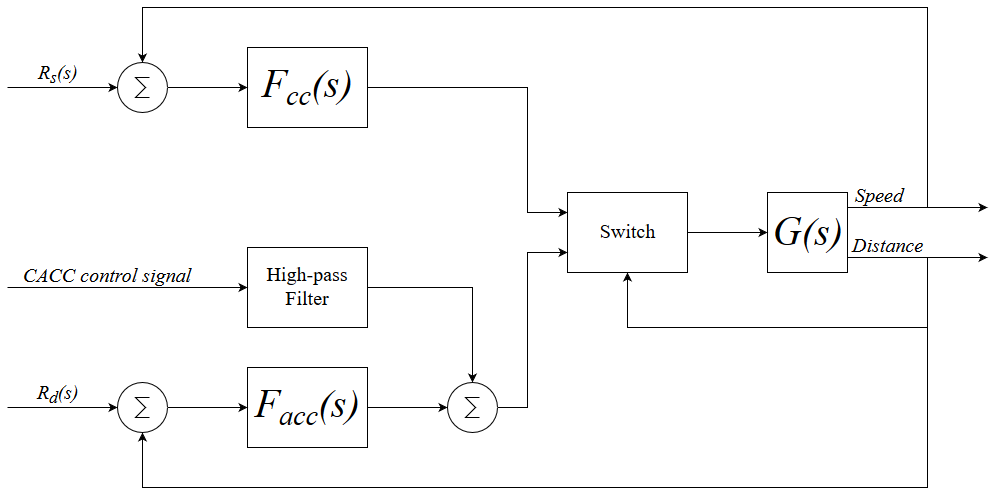
\includegraphics[width=\textwidth]{./img/design_cacc.png}
\caption{The architecture of the designed controller where $F_{cc}$ is a PID controller controlling the speed, $F_{acc}$ is a PID controller controlling the distance and G is the dynamics of the car.} \label{fig:cacc}
\end{figure}

For more information, see the report by Roshanghias~\cite{roshanghias2017}.

\subsection{Lateral control}
A lane-detecting algorithm will be implemented on a Raspberry Pi that will send data to the Alten MCS. The choice of Raspberry Pi was made because of the amount of open source video processing code available for the platform. For more info, see the report by Ferhatovic~\cite{ferhatovic2017}.\\

Lateral control will be implemented on the RTOS on the Alten MCS. The function receives the deviation from the center line as calculated by the lane detection algorithm from the Raspberry Pi, and calculates a control signal from this.

\subsection{Data aggregation}
This function will read wheel sensor data and calculate if the road conditions are unsafe for platooning. See the report by Hellman~\cite{hellman2017}.\\

The function will also serve as a filter for distance measurements and speed measurements for other tasks to use.

\subsection{Communication}
To maintain secure communication between the two vehicles in the platoon a communication protocol will be developed. For more information, see the report by Lerander~\cite{lerander2017}.% WiFi will be used to communicate wirelessly, and  WiFi messages will be parsed in a MicroBlaze processor in the FPGA and sent to the OS. 

%A WiFi module receives data and sends it via UART to a MicroBlaze processor on the FPGA where data is parsed and sent up to the OS via a mailbox. In the OS the mailbox is emptied and data is sent to where it is needed. The communication task then sends the data it should sent to the MicroBlaze where the data is packaged properly and sent as an UDP packet via the WiFi module. 

\section{Hardware implemented functions}
This section will describe the functions to be implemented on the FPGA, also known as IPs.

\subsection{Speed reading}
To read the speed of the vehicle, encoders need to be connected to the wheels. The four encoders will send pulses very quickly and a hardware decoder is needed to process them and send the speed of each wheel to the OS.

\subsection{Distance reading}
To read the distance to the preceding vehicle, a LIDAR (LIght Detection And Ranging) will be used. The LIDAR communicates the distance it is reading via a PWM signal. A hardware function is needed to read the PWM pulse and convert it to a distance.

\subsection{Communication}
WiFi communication is used between the two vehicles in the platoon. To read packages, a WiFi module is used that communicates via UART with the Alten MCS. A MicroBlaze in the FPGA processes the packages and sends the parsed data to the OS via a mailbox. For more information, see the report by Lerander~\cite{lerander2017}.

\subsection{Actuation}
To actuate control signals and thereby control the speed of the motor and the position of the steering servo, Pulse Width Modulation (PWM) is used. Two hardware implemented PWM functions will be needed for this.

\subsection{Raspberry Pi communication}
To receive information from the Raspberry Pi, some form of communication interface needs to be used. One simple solution for this is UART (Universal Asynchronous Receiver Transmitter) serial communication. 

\section{Overview design}
An overview of the different functions to be implemented on the Zynq-7000 can be seen in figure~\ref{fig:overview}.

\begin{figure}[H]
\centering
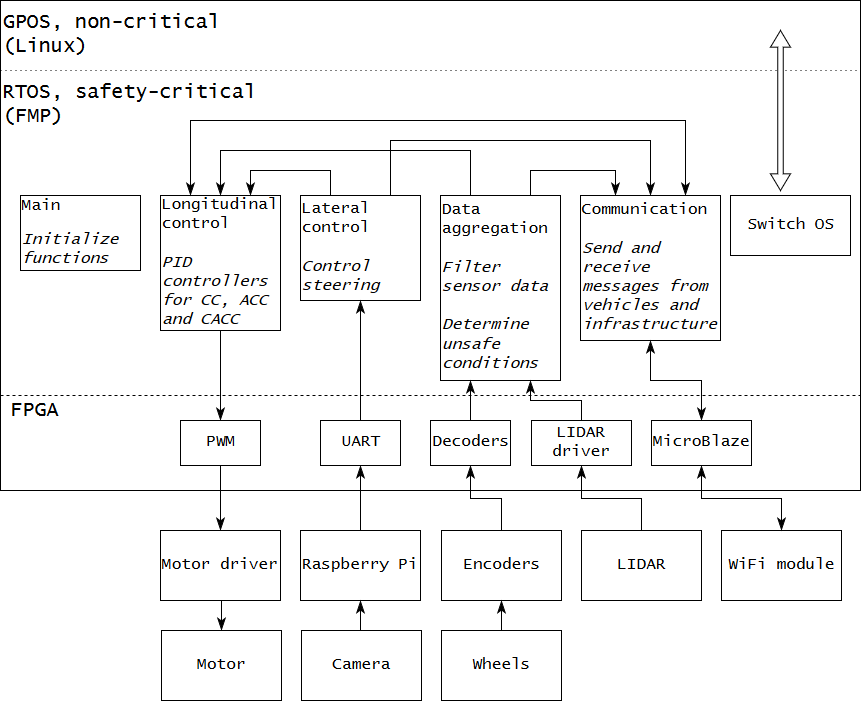
\includegraphics[width=\textwidth]{./img/design_overview.png}
\caption{Overview of the different functions to be implemented. The arrows indicate information flow between the different functions.}\label{fig:overview}
\end{figure}

A sequence diagram of the various dependencies and flow of each function can be seen in figure~\ref{fig:sequence}.

\begin{figure}[H]
\centering
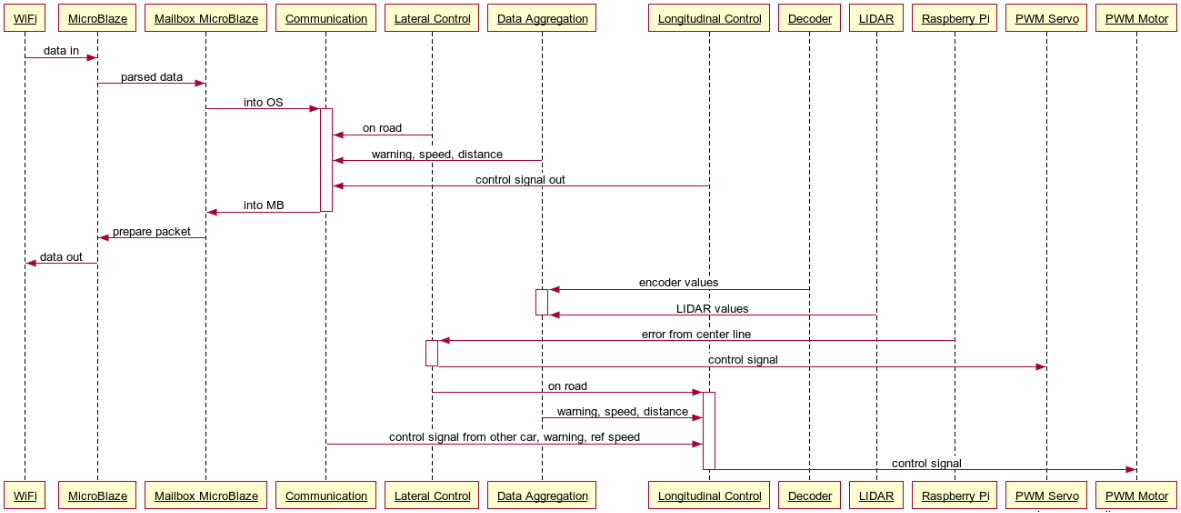
\includegraphics[width=\textwidth]{./img/design_sequence3.png}
\caption{Sequence diagram of the various hardware and software functions, their dependencies and flow of information.}\label{fig:sequence}
\end{figure}
